  \subsection{Análisis de la distorsión armónica producida por un amplificador}
    Se propone analizar un amplificador transistorizado de 4 etapas. Se ha tratado 
    en las experiencias anteriores la \textbf{alinealidad} de éste tipo de dispositivos, 
    para el presente experimento, nuevamente se debe tener en cuenta. 

    Un amplificador tiene comportamiento lineal bajo determinadas condiciones, entre ellas, 
    para pequeña señal y trabajando a lazo cerrado. Sucede que al trabajar en lazo abierto y 
    a máxima excursión, se ingresa en zonas no lineales de la función de transferencia, lo que 
    modifica el comportamiento del amplificador, provocando lo que se denomina 
    \textbf{Distorsión Armónica}.

    En la experiencia se determina el porcentaje de contenido armónico, tanto para lazo 
    abierto como para lazo cerrado, utilizando la 
    herramienta de análisis en frecuencia del osciloscopio. El circuito a implementar 
    se enseña en la Figura~\ref{fig:Exp7EsquemaCircuito}.

      \begin{figure}[H]
        \centering
          \frame{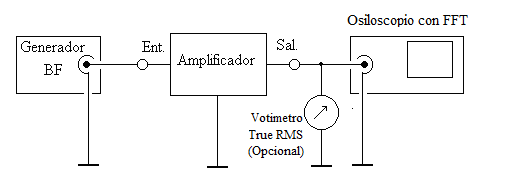
\includegraphics[width=0.8\textwidth]{Imagenes/ActividadPractica/7AnalisisDeDistorisonArmonicaEnAmpli/EsquemaConexionAmplificador.png}}
          \caption{Esquema del circuito a implementar.}
          \label{fig:Exp7EsquemaCircuito}
      \end{figure}

    En la Figura~\ref{fig:Exp7Circuito} se muestran los dispositivos y el 
    instrumental a usar.

      \begin{figure}[H]
        \centering
        \begin{subfigure}[H]{0.48\textwidth}
          \frame{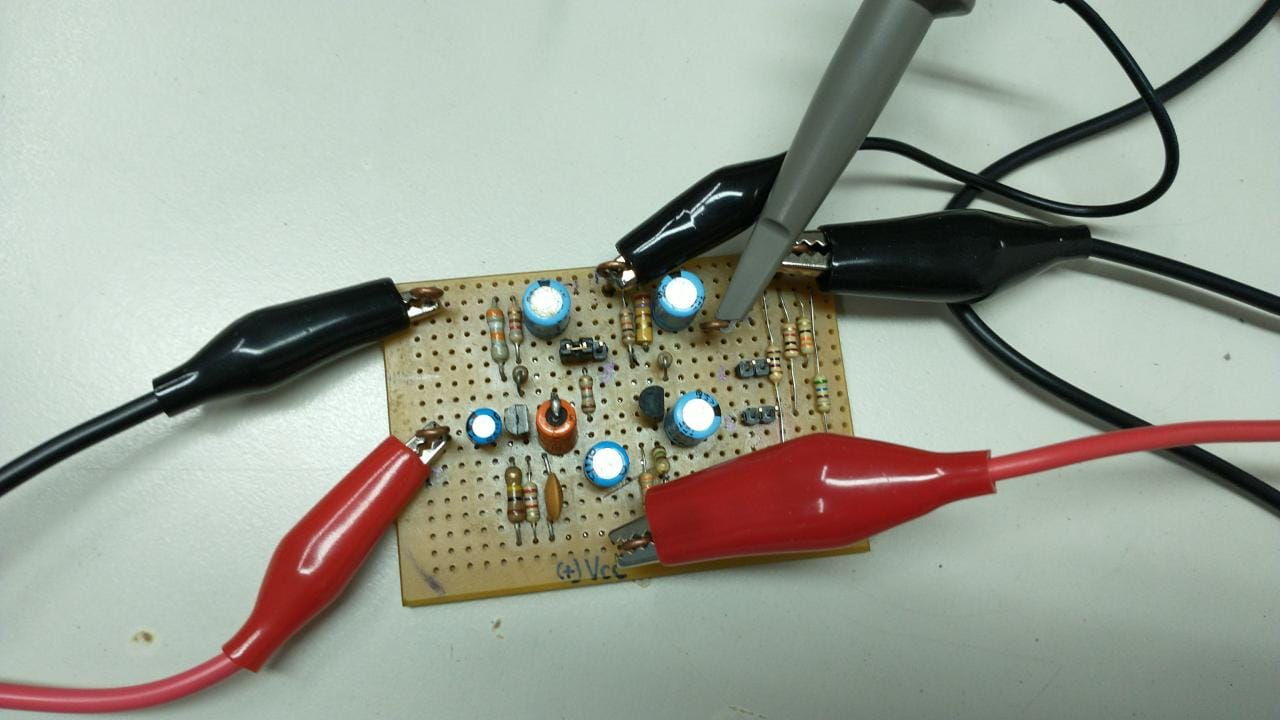
\includegraphics[width=0.8\textwidth]{Imagenes/ActividadPractica/7AnalisisDeDistorisonArmonicaEnAmpli/Amplificador.jpeg}}
          \caption{Amplificador a utilizar.}
          \label{fig:Exp7Amplificador}
        \end{subfigure}
        \hfill 
        \begin{subfigure}[H]{0.48\textwidth}
          \frame{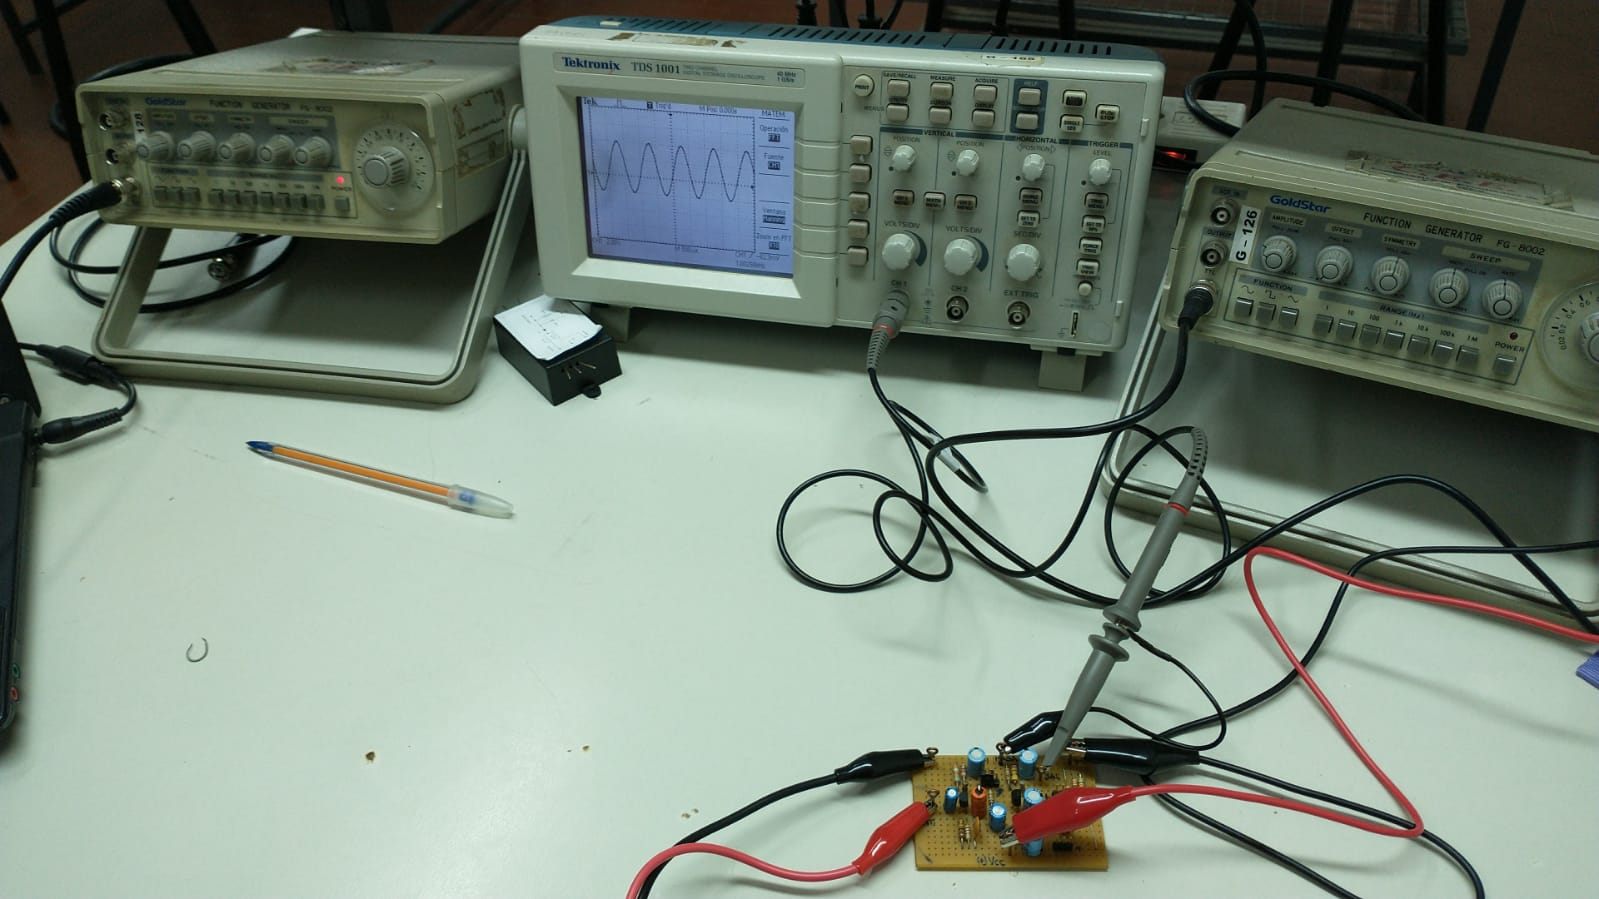
\includegraphics[width=0.8\textwidth]{Imagenes/ActividadPractica/7AnalisisDeDistorisonArmonicaEnAmpli/Equipo.jpeg}}
          \caption{Instrumental a utilizar.}
          \label{fig:Exp7Instrumental}
        \end{subfigure} 

          \caption{Amplificador a utilizar.}
          \label{fig:Exp7Circuito}
      \end{figure} 

    Inicialmente se configura el generador para \textbf{MES} (máxima excursión simétrica), y 
    una frecuencia de $\mathbf{1~kHz}$. Para ello se procede a variar la amplitud del generador hasta 
    el punto donde hay un recorte visible en la señal. La Figura~\ref{fig:Exp7MESLazoAbierto} 
    muestra dicho punto de máxima excursión.

      \begin{figure}[H]
        \centering
          \frame{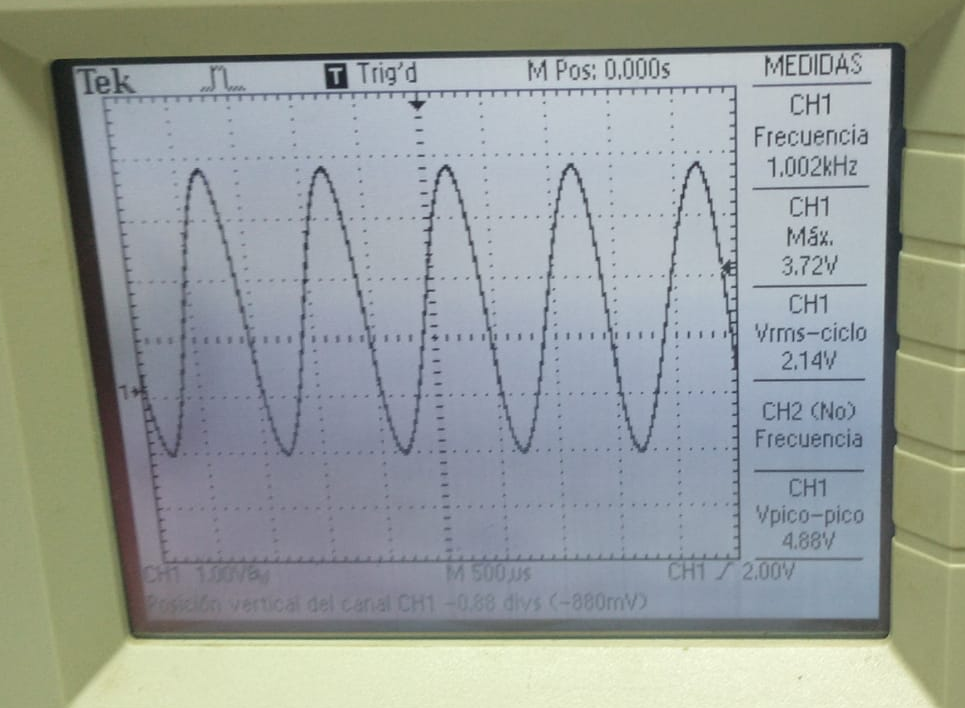
\includegraphics[width=0.48\textwidth]{Imagenes/ActividadPractica/7AnalisisDeDistorisonArmonicaEnAmpli/Exp7_MESlazoAbierto.png}}
          \caption{Máxima excursión simétrica a lazo abierto.}
          \label{fig:Exp7MESLazoAbierto}
      \end{figure}

      Luego, se procede a hacer un análisis de frecuencia, para ello se configura el osciloscopio nuevamente 
      en modo \textbf{FFT}, \textbf{Flattop}, \textbf{Zoom X10}, y $\mathbf{100~kS/s}$. En éste punto, se procede 
      a realizar la medición de la frecuencia de la fundamental y sus dos primeros armónicos, lo cual se observa en la 
      Figura~\ref{fig:Exp7FrecFundYArmonicas}.

      \begin{figure}[H]
        \centering
        \begin{subfigure}[H]{0.48\textwidth}
          \frame{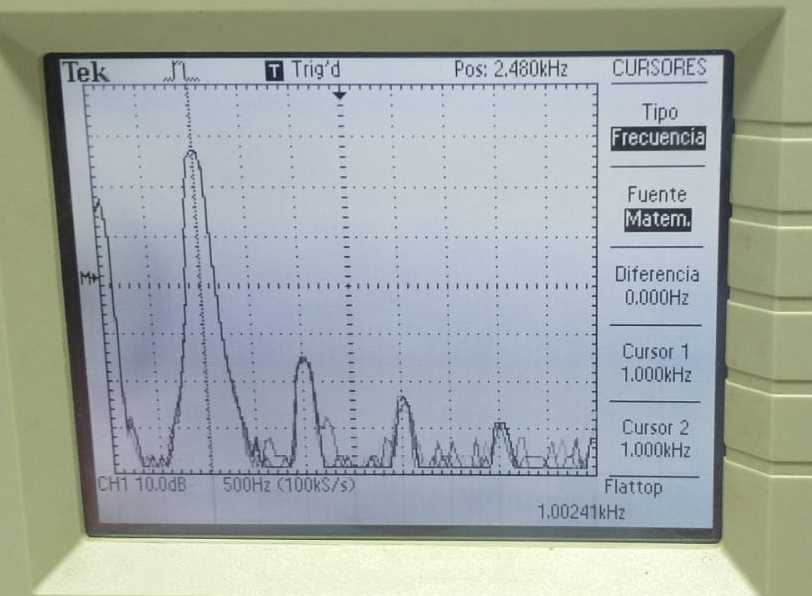
\includegraphics[width=\textwidth]{Imagenes/ActividadPractica/7AnalisisDeDistorisonArmonicaEnAmpli/Exp7_EspectroLazoAbiertoConCursorEn1k.png}}
          \caption{Frecuencia de la fundamental $f_{fund}=1~kHz$.}
          \label{fig:Exp7FrecFundamental}
        \end{subfigure}
        \hfill 
        \begin{subfigure}[H]{0.48\textwidth}
          \frame{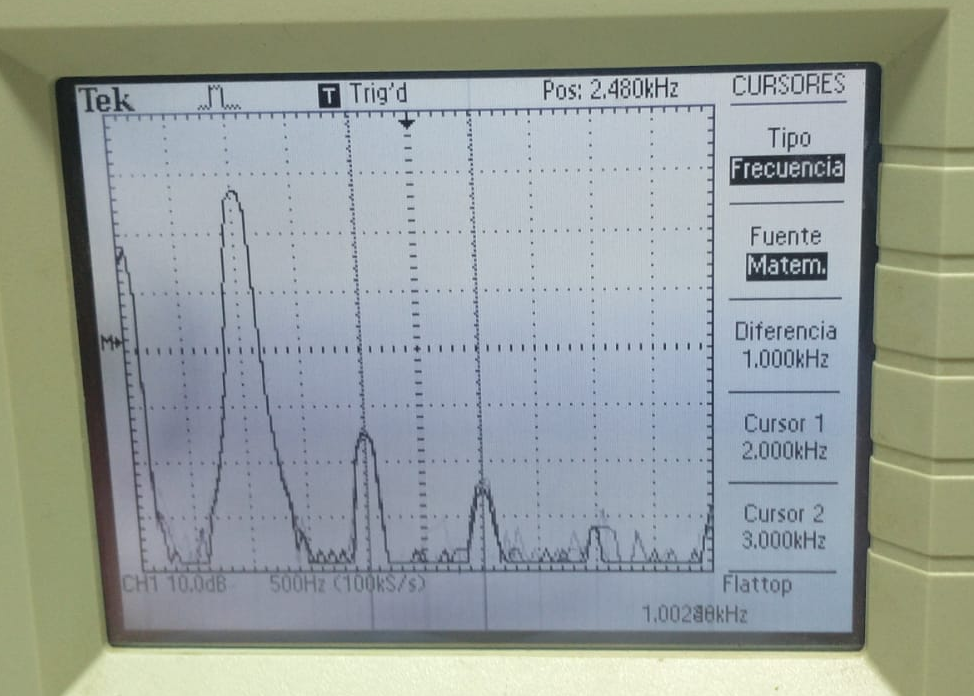
\includegraphics[width=\textwidth]{Imagenes/ActividadPractica/7AnalisisDeDistorisonArmonicaEnAmpli/Exp7_FrecuenciasDeLaSegundaYTercerArmonica.png}}
          \caption{Frecuencias de la segunda y tercer armónica $f_{2}=2~kHz$ y $f_{3}=3~kHz$.}
          \label{fig:Exp7Frec2da3raArmo}
        \end{subfigure}     
        \caption{Análisis espectral del amplificador con señal de $1~kHz$ a lazo abierto.}
        \label{fig:Exp7FrecFundYArmonicas}
      \end{figure}

      En la Figura~\ref{fig:Exp7AmplFundYArmonicasLA}, se miden las amplitudes de la fundamental y sus 
      dos primeros armónicos.

    \begin{figure}[H]
        \centering
        \begin{subfigure}[H]{0.48\textwidth}
          \frame{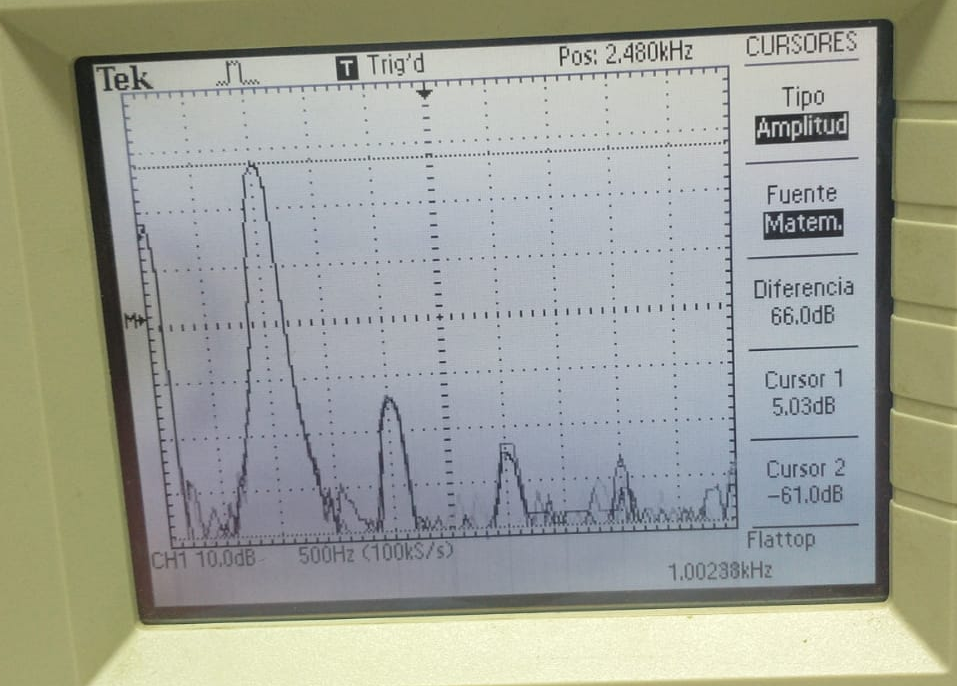
\includegraphics[width=\textwidth]{Imagenes/ActividadPractica/7AnalisisDeDistorisonArmonicaEnAmpli/Exp7_AmplitudDeLaFundamental.png}}
          \caption{Fundamental $V_{fund}=5,03~dBv$.}
          \label{fig:Exp7AmpFundamentalLA}
        \end{subfigure}
        \hfill 
        \begin{subfigure}[H]{0.48\textwidth}
          \frame{\includegraphics[width=\textwidth]{Imagenes/ActividadPractica/7AnalisisDeDistorisonArmonicaEnAmpli/Exp7_AmplitudDelSegundoArmónico.png}}
          \caption{2da armónica $V_{2da}=-37,4~dBv$.}
          \label{fig:Exp7AmpSegundaLA}
        \end{subfigure}     
        \begin{subfigure}[H]{0.48\textwidth}
          \frame{\includegraphics[width=\textwidth]{Imagenes/ActividadPractica/7AnalisisDeDistorisonArmonicaEnAmpli/Exp7_AmplitudDelTercerArmónicoALazoAbierto.png}}
          \caption{3ra armónica $V_{2da}=-47~dBv$.}
          \label{fig:Exp7AmpTercerLA}
        \end{subfigure}   
        \caption{Amplitud de la fundamental y sus dos primeras armónicas a lazo abierto.}
        \label{fig:Exp7AmplFundYArmonicasLA}
      \end{figure}

      Ahora, se procede a hacer el mismo análisis a lazo cerrado. Para empezar, se restituye el nivel de la 
      fundamental, y se ubican las frecuencias 
      de la misma y sus dos primeros armónicos, ésto se enseña en la Figura~\ref{fig:Exp7FrecLazoCerrado}.

      \begin{figure}[H]
        \centering
          \frame{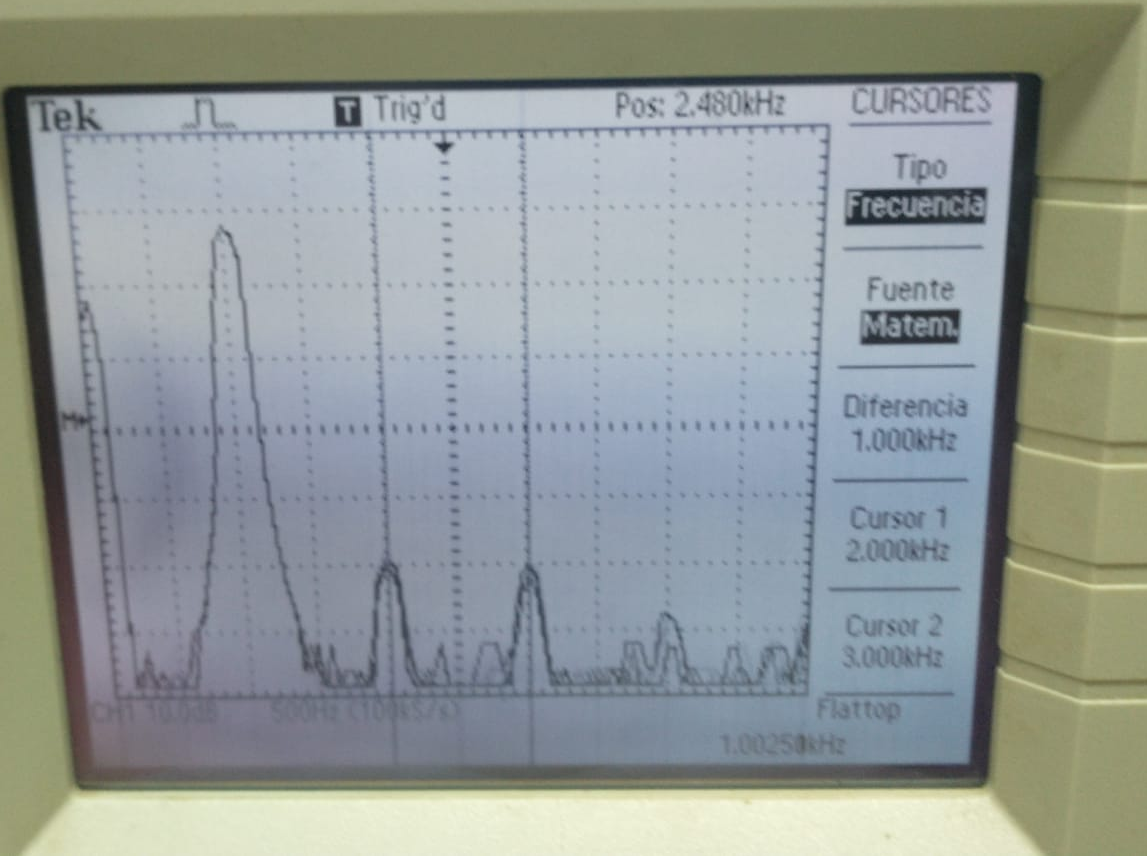
\includegraphics[width=0.48\textwidth]{Imagenes/ActividadPractica/7AnalisisDeDistorisonArmonicaEnAmpli/Exp7_LazoCerradoFrecuenciasDeSegundoYTercerArmonico.png}}
          \caption{Frecuencia de armónicos a lazo cerrado.}
          \label{fig:Exp7FrecLazoCerrado}
      \end{figure}

      Por consiguiente, se miden las amplitudes de los ya mencionados, como muestra la 
      Figura~\ref{fig:Exp7AmplFundYArmonicasLC}. Para ello se coloca un cursor en el punto 
      a medir, y éste valor es correspondiente a la amplitud en dB referenciada a $1~[V_{rms}]$.

      \begin{figure}[H]
        \centering
        \begin{subfigure}[H]{0.48\textwidth}
          \frame{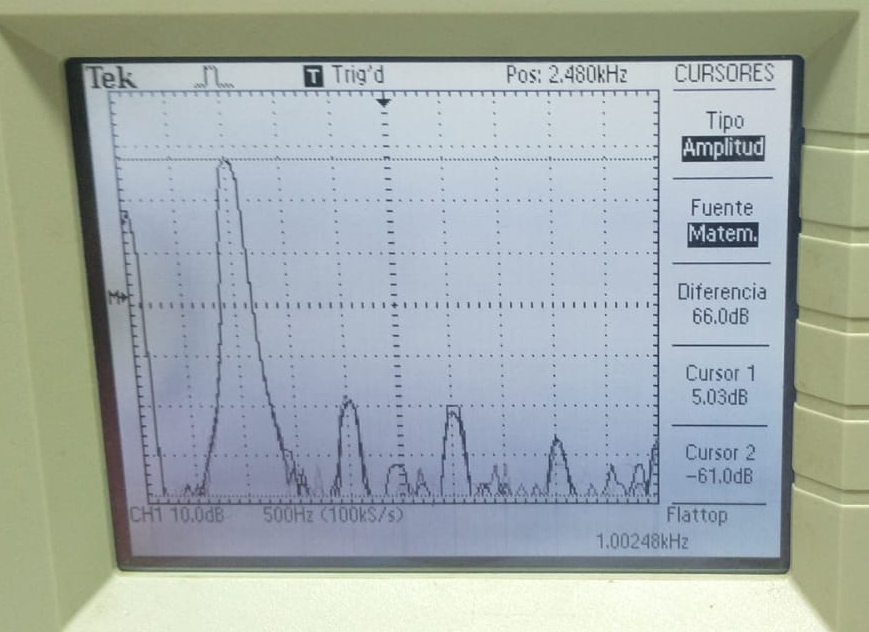
\includegraphics[width=\textwidth]{Imagenes/ActividadPractica/7AnalisisDeDistorisonArmonicaEnAmpli/Exp7_LazoCerradoAmplitudDelPrimerArmonico.png}}
          \caption{Fundamental $V_{fund}=66~dBv$.}
          \label{fig:Exp7AmpFundamentalLC}
        \end{subfigure}
        \hfill 
        \begin{subfigure}[H]{0.48\textwidth}
          \frame{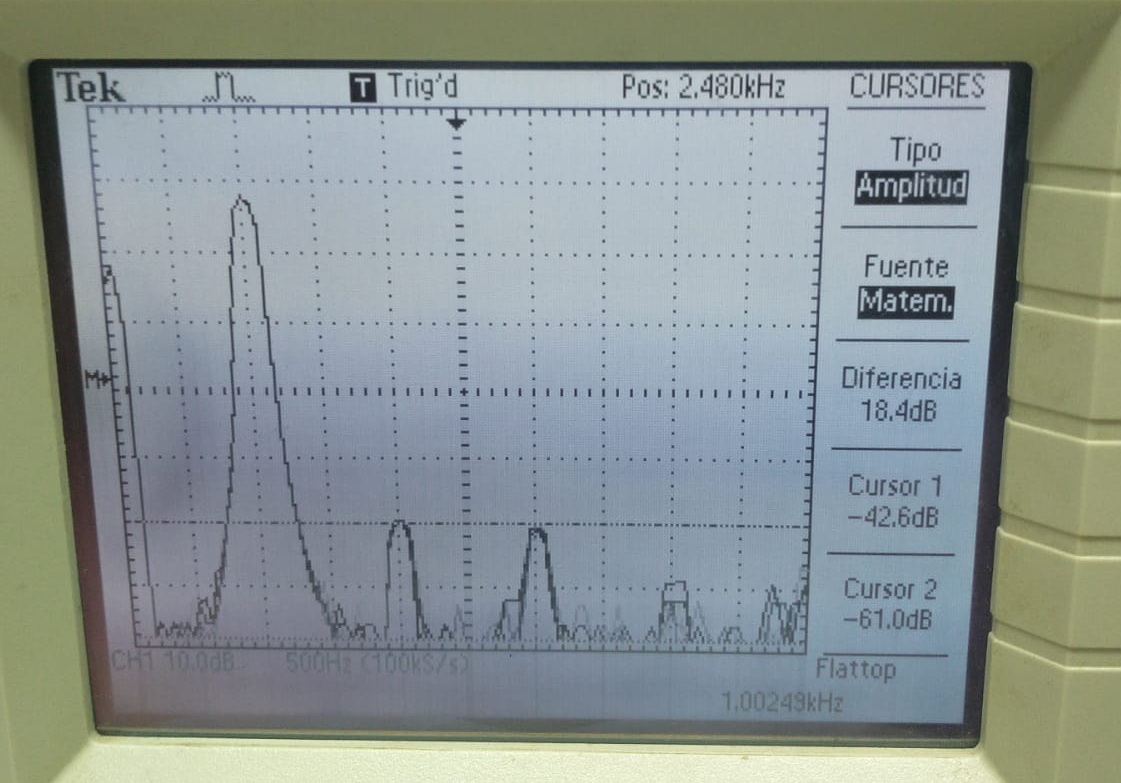
\includegraphics[width=\textwidth]{Imagenes/ActividadPractica/7AnalisisDeDistorisonArmonicaEnAmpli/Exp7_LazoCerradoAmplitudDelSegundoArmonico.png}}
          \caption{2da armónica $V_{2da}=18,4~dBv$.}
          \label{fig:Exp7AmpSegundaLC}
        \end{subfigure}     
        \begin{subfigure}[H]{0.48\textwidth}
          \frame{\includegraphics[width=\textwidth]{Imagenes/ActividadPractica/7AnalisisDeDistorisonArmonicaEnAmpli/Exp7_LazoCerradoAmplitudDelTercerArmónico.png}}
          \caption{3ra armónica $V_{2da}=16,4~dBv$.}
          \label{fig:Exp7AmpTercerLC}
        \end{subfigure}   
        \caption{Amplitud de la fundamental y sus dos primeras armónicas a lazo cerrado.}
        \label{fig:Exp7AmplFundYArmonicasLC}
      \end{figure}    

      Finalmente se confecciona una tabla de valores con los resultados obtenidos para lazo abierto y 
      lazo cerrado, y se calcula la 
      \textbf{Distorsión armónica} (DA) en porcentaje, que se define como 
        \begin{equation}
          DA_{\%}= \dfrac{V_{arm}}{V_{1}} \cdot 100~, \vspace{10pt} con~V_{arm}=\sqrt[]{V_{2da}^2+V_{3ra}^2}~.
          \label{eqn:DistorsionArmonica}
        \end{equation}
      
      Lo anteriormente dicho se muestra en la 
      Tabla~\ref{tab:Exp7DistArmLA} y la Tabla~\ref{tab:Exp7DistArmLC}.

      \begin{table}[H]
      \centering
        \begin{tabular}{ccccc} \hline \hline
          \textbf{Magnitud}            &   $\mathbf{V_{salida(PAP)}}$  &  $\mathbf{1erArmonica}$  & $\mathbf{2daArmonica}$  & $\mathbf{3raArmonica}$\\ \hline \hline
          \textbf{Frecuencia~[kHz]}    &   $1$                         &    $1$                   &   $2$                   & $3$ \\ \hline
          \textbf{dBv}                 &   $-$                         &    $5,03$                &   $-37,4$                & $-47$ \\ \hline
          \textbf{Tensión~[V]}         &   $4,88$                      &    $1,784$             &   $0,0135$              & $0,00447$\\ \hline \hline
          \end{tabular}
          \caption{Valores obtenidos a Lazo Abierto.}
          \label{tab:Exp7DistArmLA}
      \end{table}

     \begin{table}[H]
      \centering
        \begin{tabular}{ccccc} \hline \hline
          \textbf{Magnitud}            &   $\mathbf{V_{salida(PAP)}}$  &  $\mathbf{1erArmonica}$  & $\mathbf{2daArmonica}$  & $\mathbf{3raArmonica}$\\ \hline \hline
          \textbf{Frecuencia~[kHz]}    &   $1$                         &    $1$                   &   $2$                   & $3$ \\ \hline
          \textbf{dBv}                 &   $-$                         &    $5,03$                &   $-42,6$                & $-44,6$ \\\hline
          \textbf{Tensión~[V]}         &   $4,88$                      &    $1,784$             &   $0,00741$              & $0,00588$\\ \hline \hline
          \end{tabular}
          \caption{Valores obtenidos a Lazo Cerrado.}
          \label{tab:Exp7DistArmLC}
      \end{table}

      Finalmente, se determina la distorsión armónica total a lazo abierto y lazo 
      cerrado. A lazo abierto se tiene que 
      \begin{align*}
        V_{arm_{Lazo Abierto}}=\sqrt[]{(13,5~mV)^2+(4,47~mV)^2} \hspace{20pt} \Longrightarrow \hspace{20pt} V_{arm}=14,22~[mV]~,
      \end{align*}
      y haciendo uso de la ecuación~\ref{eqn:DistorsionArmonica} dicho valor será
      \begin{align*}
        Distorsion~Armonica_{arm_{Lazo Abierto}}= \dfrac{14,22~mV}{1,784~V} \cdot 100 \hspace{20pt} \therefore \hspace{20pt} \boxed{Distorsion_{LA}=0,8\%}~.
      \end{align*}

      Luego se repiten los cálculos para lazo cerrado, obteniéndose 
      \begin{align*}
        V_{arm_{Lazo Cerrado}}=\sqrt[]{(7,41~mV)^2+(5,88~mV)^2} \hspace{20pt} \Longrightarrow \hspace{20pt} V_{arm}=9,46~[mV]~,
      \end{align*}
      y con éste valor se determina la distorsión armónica total, que será 
      \begin{align*}
        Distorsion~Armonica_{arm_{Lazo Cerrado}}= \dfrac{9,46~mV}{1,784~V} \cdot 100 \hspace{20pt} \therefore \hspace{20pt} \boxed{Distorsion_{LC}=0,53\%}~.
      \end{align*}
